\chapter{Results}%
\label{chap:results}
\textit{This chapter presents various robot environments and tasks that challenge the proposed framework. The test results provide evidence that supports the answers to the research questions. The chapter starts by presenting metrics that measure task performance, the simulation environment is introduced, then a number of system models is presented and tuning variables are specified. With the system models defined and tuning parameters set test are presented, a randomized environment that is split in task that mainly involve driving and tasks that mainly involve pushing. The chapter finishes with a comparison with the state-of-the-art in \Cref{sec:compare_with_related_papers}.\bs}

\paragraph{Metrics to Measure Task Performance}
The proposed frameworks task performance is measured in metrics, these include the \ac{PE}, search-, execute- and total time to complete a task. We can draw conclusions from the evolution of the metrics over time. Furthermore, the test metrics will be used to compare the proposed framework to state-of-the-art. Now, the test metrics are presented in~\Cref{table:proposed_test_metrics}.\bs

\noindent
\begin{table}[H]
\caption{Testing metrics employed to measure task performance by the proposed robot framework in the left column. Motivation on relevance of the metric is provided in the corresponding right column.}\label{table:proposed_test_metrics}
\centering
\begin{tabular}%
  {>{\raggedright\arraybackslash}p{0.25\textwidth}%
   >{\raggedright\arraybackslash}p{0.65\textwidth}}
\acl{PE} [meter] &  The \ac{PE} is high in two scenario's, first when unexpected behaviour occurs, second when the system model used to calculate the \ac{PE} describes the system poorly. When the \ac{PE} is low, that would indicate the robot encounters expected behaviour and that the model describes the system accurate. If the \ac{PE} is lowering during task execution over time, that would indicating the robot is learning to select models that are more accurate and less unexpected behavior occurs.\\
% Total Average\newline \acl{TE}& The total average \ac{TE} is created by averaging over every hypothesis' average \ac{TE} in a \ac{h-graph}. Seeing the total average \ac{TE} lower over time would indicate the robot is selecting better suitable controllers and system models, indicating the robot is learning.\\
% Final poses and\newline displacement errors & The final pose and displacement error is a metric which how a controller performs. This thesis does not create or investigate controllers, but it is interesting to see why different controllers are preferred for different objects. The final pose and displacement error could be the cause.\\
% The ratio between the number of hypotheses and the number of tasks & Expected is that whilst learning system models, the hypothesis created will be more effective. Thus the ratio between the total number of hypotheses and the total number of tasks is expected to lower with new knowledge.\\
% The ratio between the number of successful and the number of total edges in \ac{k-graph} & When the \ac{k-graph} improves recommending a controller and system model, the ratio between successful edges and total edges is expected to increase because, with better recommendations, more edges will be completed.\\
search time [sec]& The time the proposed framework spends searching for hypotheses. The search time is dominated by path planning because compared to path estimation, updating the \ac{h-graph} it is time consuming. The number of subtasks in a task, the environment and the number of unknown and classified objects influence the number of paths to be planned and the duration of planning, and thus the search time.\\ 
execution time [sec] & The time the proposed framework spends executing hypotheses. The execution time is dominated by path length, driving or pushing toward a target pose on the other side of the workspace takes more time compare to a target pose closeby the initial pose.\\ 
total time [sec] & search time + execution time.\\
\end{tabular}
\end{table}

\paragraph{The Simulation Environment}
Testing in a simulation environment has been done using the URDF Gym Environment~\cite{spahn_urdfenvironment_2022}, a 100\% python environment build upon the PyBullet library~\cite{coumans_pybullet_2016}. The code created during the thesis can be found on \href{https://gitlab.tudelft.nl/airlab-delft/msc_projects/msc_gijs_groote}{GitLab} and \href{https://github.com/GijsGroote/semantic-thinking-robot}{GitHub}. Experiments are taken on laptop with specifications: Laptop: HP ZBook Studio x360 G5, OS:~Ubuntu 22.04.1 LTS x86\_64, CPU: Intel i7-8750H (12) @ 4.100GHz, GPU: NVIDIA Quadro P1000 Mobile. The simulation environment provides many different robots, of which one robot is selected to perform tests, the point robot, which is are displayed in \Cref{fig:example_robots}. The point robot takes an velocity input along the \gls{x}- and in \gls{y}-axis.\bs

Robot input is defined as:\\
\[ u(k) = {[ u_{\gls{x}}(k), u_{\gls{y}}(k) ]}^\top \]

During testing three controllers have been used. A \ac{MPC} and \ac{MPPI} controller for driving the robot named \textit{mpc-drive-controller} and \textit{mppi-drive-controller}, and a \ac{MPPI} controller for robot pushing named \textit{mppi-push-controller}. The \ac{MPC} and \ac{MPPI} control methods were introduced in \Cref{sec:control_methods}. Three system models are developed without drawing upon any existing source material. The first model is an \ac{LTI} model describing robot driving, the second model is an \ac{LTI} model describing robot the robot pushing an object, the third model is a nonlinear model also describing robot pushing. First a short textual description of the available system models is provided below. Second, the state-space model is provided for the three implemented models.\bs

\begin{table}[H]
\caption{The left column displays the available models of drive- and push systems, accompanied by a description in the corresponding right column.}\label{table:available_system_models}
\centering
\begin{tabular}%
  {>{\raggedright\arraybackslash}p{0.25\textwidth}%
   >{\raggedright\arraybackslash}p{0.65\textwidth}}
\textit{lti-drive-model} & A second order \ac{LTI} model that is compatible with both the \ac{MPC} and the \ac{MPPI} drive controller. The state variables are the robot's \gls{x} and \gls{y} position. The next state $x(k+1)$ is based on the current state $x(k)$, the time step \gls{DT} and robot system input $u(k)$.\\
\textit{lti-push-model} & A \ac{LTI} model that is compatible with only the \ac{MPPI} push controller. The state variables are the robot's and the pushed object's \gls{x} and \gls{y} position. The next state $x(k+1)$ is based on the current state $x(k)$, the time step \gls{DT} and robot system input $u(k)$.\\
\textit{nonlinear-push-model} & 
A nonlinear model that is compatible with only the \ac{MPPI} push controller. The state variables are the robot's and the pushed object's \gls{x} and \gls{y} position and the objects orientation $\gls{theta}_\mathit{obj}$. The next state $x(k+1)$ is based on the current state $x(k)$, the time step \gls{DT}, robot system input $u(k)$ and geometrical variables $v_p$ and $s_t$.\\
\end{tabular}
\end{table}

State-space representation of the \textit{lti-drive-model}:\bs

\begin{equation}
\label{eq:lti-drive-model}
x_{\mathit{lti-drive-model}}(k+1)=
\begin{bmatrix}
\gls{x}_\mathit{robot}(k+1)\\
\gls{y}_\mathit{robot}(k+1)
\end{bmatrix}
=
\begin{bmatrix}
\gls{x}_{\mathit{robot}}(k) + \gls{DT} u_{\gls{x}}(k)\\
\gls{y}_{\mathit{robot}}(k) + \gls{DT} u_{\gls{y}}(k)
\end{bmatrix}
\end{equation}

State-space representation of the \textit{lti-push-model}:\bs

\begin{equation}
x_{\mathit{lti-push-model}}(k+1)=
\begin{bmatrix}
\gls{x}_{\mathit{robot}}(k+1)\\
\gls{y}_{\mathit{robot}}(k+1)\\
\gls{x}_{\mathit{obj}}(k+1)\\
\gls{y}_{\mathit{obj}}(k+1)
\end{bmatrix}
=
\begin{bmatrix}
\gls{x}_{\mathit{robot}}(k+1) + \gls{DT} u_{\gls{x}}(k)\\
\gls{y}_{\mathit{robot}}(k+1) + \gls{DT} u_{\gls{y}}(k)\\
\gls{x}_{\mathit{obj}}(k+1) + \frac{1}{2} \gls{DT} u_{\gls{x}}(k)\\
\gls{y}_{\mathit{obj}}(k+1) + \frac{1}{2} \gls{DT} u_{\gls{y}}(k)
\end{bmatrix}
\label{eq:lti-push-model}
\end{equation}


State-space representation of the \textit{nonlinear-push-model}:\bs
\begin{equation}
x_{\mathit{nonlinear-push-model}}(k+1)=
\begin{bmatrix}
\gls{x}_{\mathit{robot}}(k+1)\\
\gls{y}_{\mathit{robot}}(k+1)\\
\gls{x}_{\mathit{obj}}(k+1)\\
\gls{y}_{\mathit{obj}}(k+1)\\
\gls{theta}_{\mathit{obj}}(k+1)
\end{bmatrix}
=
\begin{bmatrix}
\gls{x}_{\mathit{robot}}(k) + \gls{DT} u_{\gls{x}}(k)\\
\gls{y}_{\mathit{robot}}(k) + \gls{DT} u_{\gls{y}}(k)\\
\gls{x}_{\mathit{obj}}(k) + \gls{DT}\cos(\gls{theta}_{\mathit{obj}}(k)) (1-|\frac{2\mathit{s_t}}{H}|)\mathit{v_p}\\
\gls{y}_{\mathit{obj}}(k) + \gls{DT}\sin(\gls{theta}_{\mathit{obj}}(k)) (1-|\frac{2\mathit{s_t}}{H}|)\mathit{v_p}\\
\gls{theta}_{\mathit{obj}}(k) + \frac{2*\gls{DT}*\mathit{v_p}*\mathit{s_t}}{H}
\end{bmatrix}
\label{eq:nonlinear-push-model}
\end{equation}


Where distance $s_t$ and velocity $v_p$ can be visually seen in \Cref{fig:robot_and_square_object}. A positive $s_t$ indicates the object will rotate anticlockwise, a negative $s_t$ indicates a clockwise rotation. The width of an object is defined as \textit{H} and is set to 2 meters.\bs

\begin{figure}[H]
    \centering
    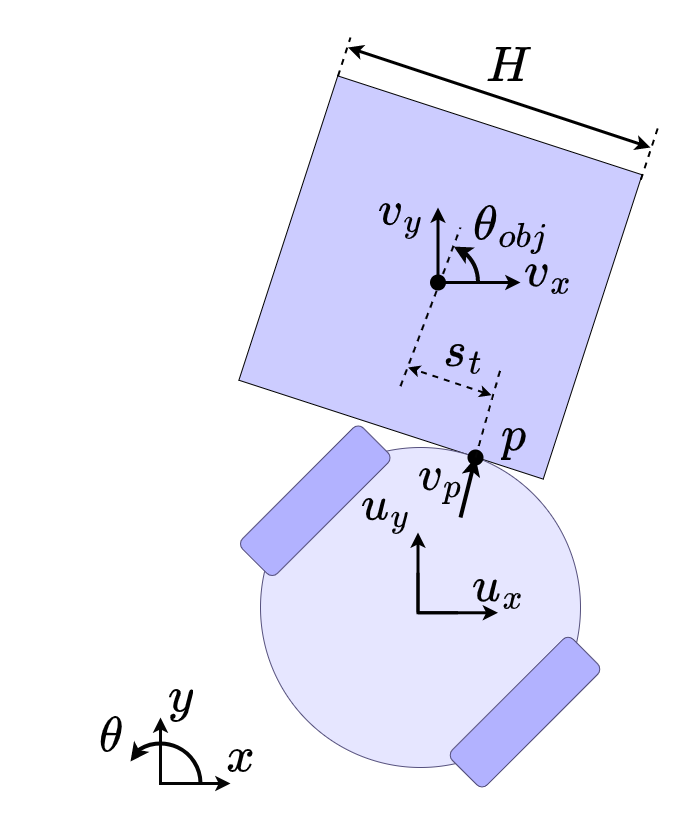
\includegraphics[width=7cm]{figures/results/robot_and_square_object.drawio}
    \caption{Schematic overview of point robot pushing a box object.}%
    \label{fig:robot_and_square_object}
\end{figure}

Where $v_p$ is the velocity of the robot perpendicular to the object defined as:\bs
\[ \mathit{v_p} = u_{\gls{x}} \cos(\gls{theta}_{\mathit{obj}}(k)) + u_{\gls{y}}\sin(\gls{theta}_{\mathit{obj}}(k)) \]

Two drive action edge parameterizations are available: (\textit{mpc-drive-controller}, \textit{lti-drive-model}) and (\textit{mppi-drive-controller}, \textit{lti-drive-model}), and two push action edge parameterizations are available: (\textit{mppi-push-controller}, \textit{lti-push-model}) and (\textit{mppit-push-controller}, \textit{nonlinear-push-model}).\bs

The goal of this thesis is not to find optimal control, or to model the environment with great accuracy. The goal is to select the best edge parameterization in the available set of edge parameterizations. Elaborating the control design and system model design is therefore out of the scope of this thesis, the control design parameters such as prediction horizon, cost function, number of rollouts can be found in the implementation.\bs

% \section{Benchmark Tests}%
% \label{sec:benchmark_tests}
% Three benchmark test are presented, starting with the blockade task. A large part of the proposed framework is system identification, for testing however no system identification is performed. Instead, several analytic system models are used, and the \ac{k-graph} finds which system model is the best choice for an object over time. Where the best choice is defined using the edge metrics discussed in \Cref{subsec:edge_metrics}. The analytic system models are not opting for modelling the drive or push model as accurately as they possibly can, thus severe model mismatch should be expected. Such model mismatch is no issue, to complete a subtask stable closed-loop control is required, when an edge parameterization is unable to provide closed-loop stable control, the edge will fail because a fault will be detected. To answer the research question, improvement over time should be made. Gaining such improvement does not require accurate system models, time spend improving the hand-coded system models does thus not change the result.\bs
%
%
% \paragraph{Blockade} In the blockade environment the robot is tasked with placing a box in a target pose that is blocked by a cylinder object.\bs
% \begin{figure}[H]
%     \centering
%     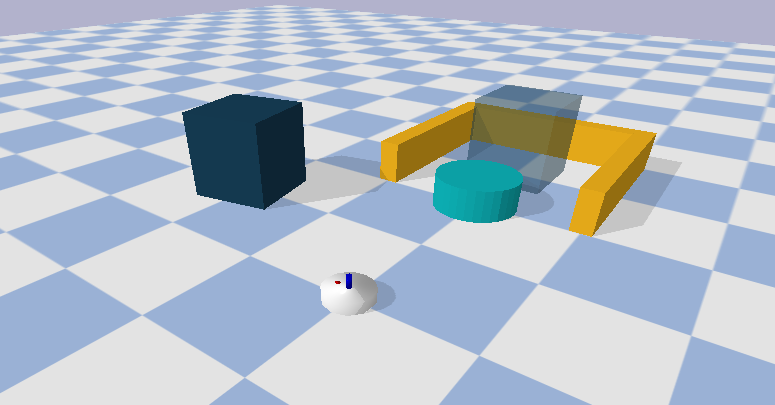
\includegraphics[width=0.9\textwidth]{figures/results/blockade}
%     \caption{The blockade environment with the target ghost pose for the blue box. The green walls are unmovable whilst both the blue box and cylinder are movable.}%
%     \label{fig:benchmark_blockade}
% \end{figure}
%
% The blockade task neatly shows that the \ac{h-algorithm} uses the backward search technique. First, the \ac{h-algorithm} plans to push the box directly to the target pose, then it realizes a blocking object must first be moved to free the path. It makes the mistake of pushing the unmovable wall, then it succeeds in pushing the movable cylinder out of the way. The \ac{k-graph} then ensures that this mistake will not occur again because is remembered that the wall is immovable. Over time the \ac{k-graph} indicates that it prefers to use the \ac{MPPI} controller with the nonlinear-push-model to push both the box and the cylinder object. Converging to this conclusion improves the testing metrics for the task as can be seen in \Cref{fig:results_blockade}\bs
%
% \todo[inline]{is nonlinear-push-model still the preferred model after testing??}
%
% \begin{figure}[H]
%     \centering
%     
\includegraphics[width=0.9\textwidth]{figures/tests/404_not_found}
%
%     \caption{Some results are still under development for the blockade environment}%
%     \label{fig:results_blockade}
% \end{figure}
% \todo[inline]{Test to create results for running the blockade environment, and input into above 404 not found}
%
% \paragraph{Swap}
% In the swap environment the robot should swap the locations of the 2 objects in the environment.\bs
%
% \begin{figure}[H]
%     \centering
%     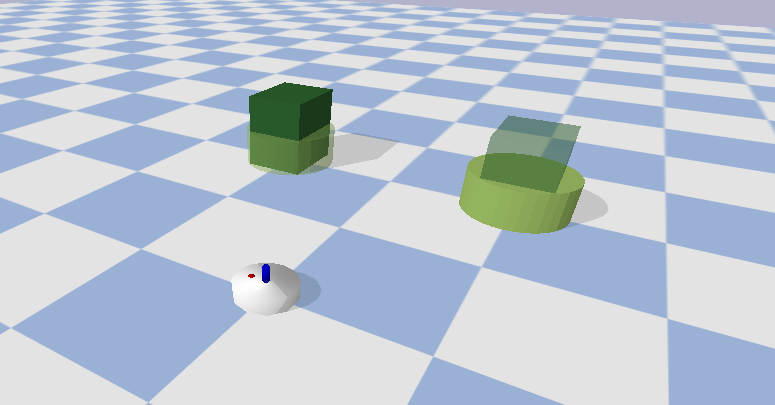
\includegraphics[width=0.9\textwidth]{figures/results/swap}
%     \caption{The swap environment, the robot is tasked with swapping the poses of the cylinder and the box.}%
%     \label{fig:benchmark_swap}
% \end{figure}
% The swap task shows that the \ac{h-algorithm} can handle overlapping subtasks. The \ac{h-algorithm} handles a single subtask at a time and randomly selects which subtask to handle next. The result for the swap task is that first, the robot will place the box on the location of the cylinder. The cylinder is blocking the path and is thus pushed to free the path, then the robot drives back to the box to push the box to its target pose. The cylinder can directly be pushed toward its target pose, because there is a free path, and the task is successfully completed. By manual inspection, this is the most efficient action sequence to complete the swap task. But there is an assumption because the initial environment has a distance between the robot and box (robot-box distance), and robot and cylinder (robot-cylinder distance) that is equal. If the initial robot-box distance is greater than the initial robot-cylinder distance, it would be more efficient to first drive toward the cylinder because that distance is smaller. The selection of subtask is random, thus there is a 50\% chance that the robot selects a subtask resulting in driving more than is necessary to complete the swap subtask.\bs
%
% \begin{figure}[H]
%     \centering
%     
\includegraphics[width=0.9\textwidth]{figures/results/404_not_found}
%     \caption{Some tests are still under development for the swap environment}%
%     \label{fig:results_swap}
% \end{figure}
%
% \todo[inline]{Test to create results for running the swap environment}
%
% \paragraph{Surrounded} In the surround environment the robot has to learn which box is movable to escape the enclosure of boxes.\bs
% \begin{figure}[H]
%     \centering
%     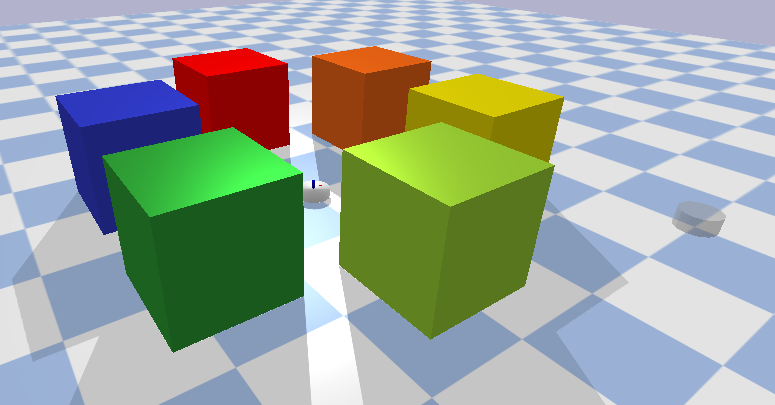
\includegraphics[width=0.9\textwidth]{figures/results/surrounded}
%     \caption{The surround environment, the robot is tasked with escaping the surrounding enclosure by driving to the target ghost pose displayed on the right side in the figure. Every box objects is unmovable except the red box which is movable.}%
%     \label{fig:benchmark_surround}
% \end{figure}
% The surround task show that having and gaining environment knowledge can greatly improve task execution. Simply knowing if an object can be interacted with may lower task execution time drastically as can be seen in \Cref{fig:results_surround}.\bs
%
% \begin{figure}[H]
%     \centering
%     
\includegraphics[width=0.9\textwidth]{figures/results/404_not_found}
%     \caption{Some test are still under development for the surround environment}%
%     \label{fig:results_surround}
% \end{figure}
%
% \todo[inline]{Test to create results for running the surround environment}

\section{Driving and Pushing Experiments}%
\label{sec:randomization}
To improve the relevance of the experimental results, driving and pushing tasks are performed with randomized settings. A set of multiple tasks is given to the robot, named a \textit{run}. When the robot is tasked with the first task in the run the \ac{k-graph} is empty, and when the last task in the run is completed the \ac{k-graph} is filled with the experience gained. For each run, a set of random objects and properties are generated. This remains the same for the whole run, however for each task in the run the environment is reshuffled. A reshuffled does three things, first, it resets the robot pose, secondly, it gives the objects in environment new initial pose. Thirdly, new target poses are generated for the subtask in the new task. By solving multiple reshuffled tasks in a reshuffled environment, the robot gains experience that is stored in the \ac{k-graph}.\bs

\Cref{table:configure_rand_env} presents a set of parameters that initializes the random environment. Two type of tasks solved by the robot, a driving task, where the robot must drive toward multiple random target poses, and a pushing task, where the robot must push a movable object toward a random target pose.\bs

\noindent
\begin{table}[H]
\caption{The tuning parameters to initialize a random environment}%
\label{table:configure_rand_env}
\centering
\begin{tabular}%
{>{\raggedright\arraybackslash}p{0.25\textwidth}%
>{\raggedright\arraybackslash}p{0.65\textwidth}}
The \textit{size of the grid} & length and width of the ground plane in \gls{x} and \gls{y} direction.\\
The \textit{minimal and maximal size of objects} & A box will have sides with a length that lie in the specified range from minimal to maximal length. Cylinders will have a diameter and height that is within the specified range, additionally, cylinders are not higher than the radius of the cylinder to prevent cylinders from tipping over. \\
The \textit{maximal weight} & which is uniformly distributed for the environment objects, minimal weight is set by default to 1 kilogram. \\
The \textit{number of unmovable objects} & Specify the amount of unmovable objects.\\
The \textit{number of movable objects} & Specify the amount of movable objects.\\
The \textit{number of subtasks in a task} & Specify the amount of subtasks in a task.\\
The \textit{number of boxes and cylinders} & For every new object generated there is a 50\% chance it becomes a box and 50\% chance it becomes a cylinder.
\end{tabular}
\end{table}

An randomly initialized environment that is then reshuffled can be visualized in \Cref{fig:random_environment_reshuffle}.\bs

\begin{figure}[H]
    \centering
    \begin{subfigure}{.49\textwidth}
    \centering
    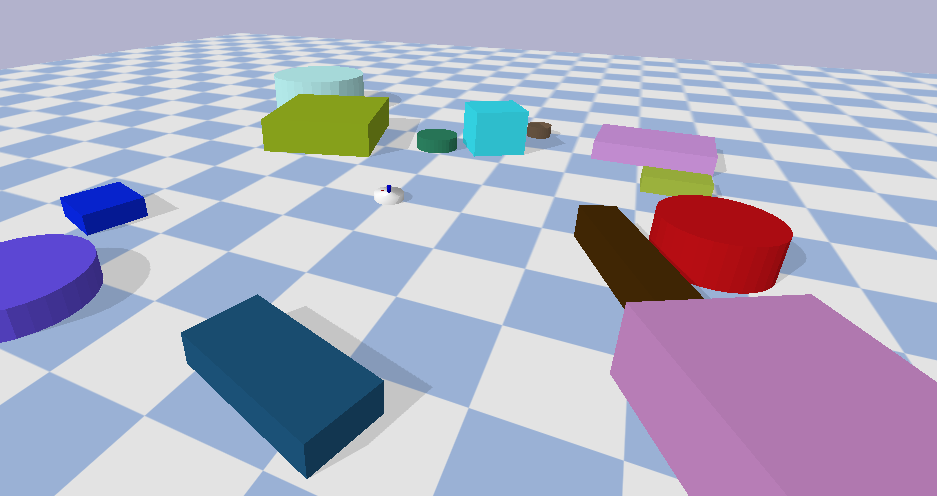
\includegraphics[width=\textwidth]{figures/results/random1}
    \caption{Environment after initialization.}
    \end{subfigure}
    \hfill
    \begin{subfigure}{.49\textwidth}
    \centering
    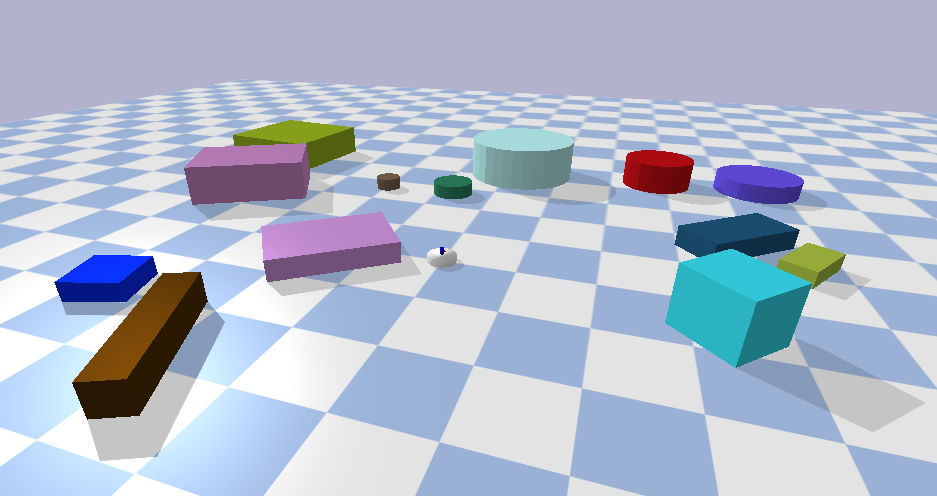
\includegraphics[width=\textwidth]{figures/results/random2}
    \caption{Environment after a reshuffle.}
    \end{subfigure}

    % \vspace{0.2cm}
    % \begin{subfigure}{.49\textwidth}
    % 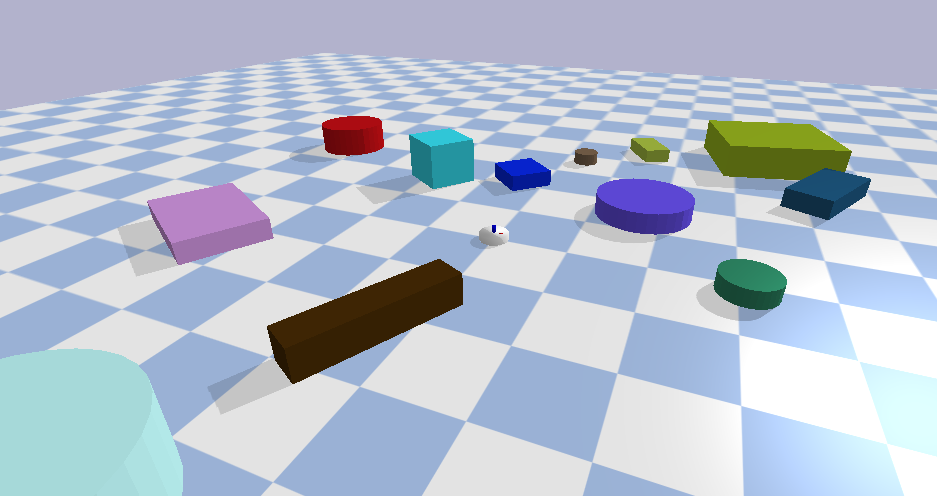
\includegraphics[width=\textwidth]{figures/results/random3}
    % \caption{Environment after second reshuffle.}
    % \end{subfigure}
    % \hfill
    % \begin{subfigure}{.49\textwidth}
    % \centering
    % 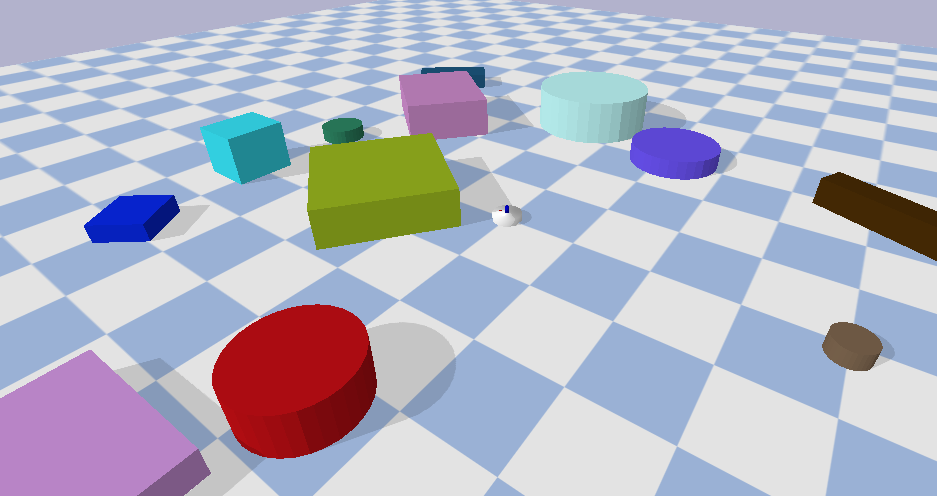
\includegraphics[width=\textwidth]{figures/results/random4}
    % \caption{Environment after thirth reshuffle.}
    % \end{subfigure}
    \caption{A random environment initialized by tuning parameters presented in \Cref{table:configure_rand_drive_env_values} and randomness.}%
    \label{fig:random_environment_reshuffle}
\end{figure}

\subsection{A Driving Task}%
\label{subsec:rand_driving}
For the driving task the random environment is created with the following tuning parameters.\bs

\begin{table}[H]
\caption{The selected tuning parameters for the randomized drive environment.}%
\label{table:configure_rand_drive_env_values}
\centering
\begin{tabular}%
{>{\raggedright\arraybackslash}p{0.30\textwidth}%
>{\raggedright\arraybackslash}p{0.60\textwidth}}
\text{grid size}  &\gls{x}=12 m, \quad \gls{y}=12 m \\
\text{object size}  &$\mathit{min\_length}=0.2 m, \quad \mathit{max\_length}=2 m$ \\
\text{object weight}  &$\mathit{max\_weight}=1000 kg$\\
\text{number of objects}  &$\mathit{num\_unmovable\_obj}=3, \quad \mathit{num\_movable\_obj}=5$ \\
\text{number of tested runs}  &$\mathit{num\_runs}=10$\\
\text{number of tasks in a run}  &$\mathit{num\_tasks}=10$\\
\text{number of subtasks in a task}  &$\mathit{num\_subtasks}=3$
\end{tabular}
\end{table}

These parameters have been specifically selected, starting with the size of the ground floor. The ground floor should be large enough such that objects can be pushed around, note that, for a driving task, pushing is involved when a path must be freed. An enormous (100 by 100 meter) ground floor would result in a longer computational time for path planning, which is undesired. A 12 by 12 meter ground floor is selected because the floor is large enough for objects to be pushed around. The range that determines the size of objects is set such that objects can be as large as the robot itself, and be around 10 times as large as the robot. With these sizes the robot is unable to grasp objects, a gripper would be too small to grasp objects. The comparatively large size fits the objective of nonprehensile pushing, there simply is no other method to manipulate such large objects other than pushing. A real-life example are can be found in harbors where tug boats push giant cargo ships around that are many times over the size of the tug boat. The ratio of solid obstacles vs.~movable objects determines if a task is more navigation (only solid obstacles) or more \ac{NAMO} (only movable objects). A task that tends toward \ac{NAMO} is favored because that is the target environment in this thesis. There should be some unmovable obstacles that reward the robot learning such objects are unmovable (to then not interact with them). Thus there are more movable objects than solid obstacles chosen, whilst still having 2 solid obstacles around. Ten runs are taken, each run consisting of 10 tasks, the results are averaged to reach statistic relevance in a randomized environments. The number of subtasks is set to 3, a low number of drive subtasks that can be completed in under 2 minutes.\bs

Lastly, a number of tuning parameters must be set for the \ac{h-algorithm}. These are the maximal robot speed, set to 1 $\frac{\mathit{meter}}{\mathit{s}}$, the \textit{cell size} for the path estimator set to 0.1 meter, the path planner takes four tuning parameters; the \textit{step size} set to 0.2 meter, the \textit{search size} set to 0.35 meter, the \textit{MovableSpaceCost} set to 2 meter and the \textit{UnknownSpaceCost} set to 3.5 meter.\bs

The search- and execution time to complete a task is investigated, and especially its development over multiple tasks. Then a comparison is made between completing reshuffled tasks once with the \ac{k-graph} that suggests edge parameterizations, and once without suggestions, by randomly selecting a available edge parameterization. Given the above parameters, all parameters are now set. Ten runs are solved by the robot where every run is composed of ten tasks. The first generated environment in the run determines the type of objects and their properties that remain unchanged for the entire run. The subsequent environments in the run are reshuffled versions of the first environment. After ten runs the task performance is collected that is expressed in the metrics just described. The ten runs metrics are vertically augmented such that they are grouped by the same number of tasks in experience. First, a boxplot is presented displaying execution-, search- and total times over the ten runs whilst using \ac{k-graph} action suggestions in \Cref{fig:random_drive_time_k-graph}. The number of solved subtasks can be calculated by multiplying the number of runs times the number task in a run by the number of subtasks in a task, which is $10 \cdot 10 \cdot 3 = 300$ subtasks. The available drive edge parameterizations that can be selected are: (\textit{mpc-drive-controller}, \textit{lti-drive-model}) and (\textit{mppi-drive-controller}, \textit{lti-drive-model}).\bs

\begin{figure}[H]
    \centering
    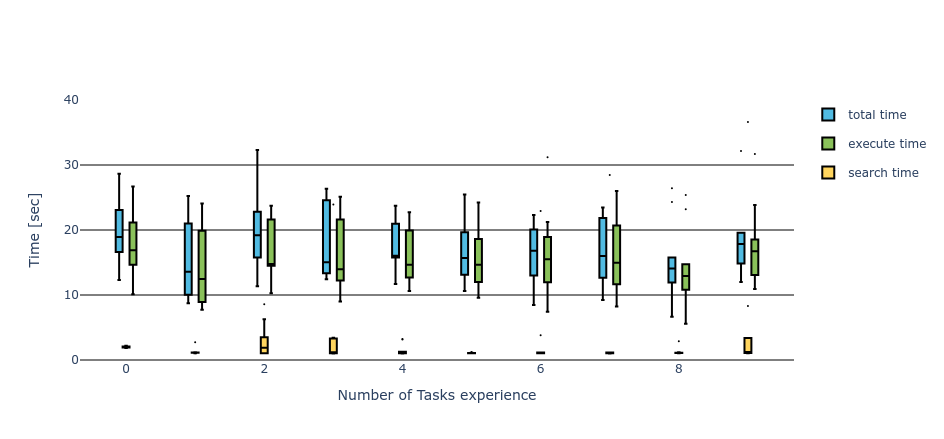
\includegraphics[width=\textwidth]{figures/results/random_drive_time_k-graph}
    \caption{Search-, execution- and total time to complete a drive task \textbf{whilst} using \ac{k-graph} action suggestions. The horizontal axis indicates the number of task experience in a run. The vertical axis displays a boxplot of the search-, execution- and total time over ten runs grouped by number of tasks in experience.}%
   \label{fig:random_drive_time_k-graph}
\end{figure}

In the above figure the \ac{h-algorithm} initially selects a random edge parameterization, also known as the learning phase. The duration of the learning phase is the first task, which can be concluded from \Cref{table:rand_drive_mpc_vs_mppi}. From that table it becomes clear that after the first task, only the \ac{MPC} parameterization is selected for driving tasks, indicating the learning phase is over. Since the learning phase is already over after the first task, it is hard to identify a trend in search-, execute- or total time during learning, because there is only one data point in the learning phase. After the learning phase, in the converging phase starts, the total execution time deviates between 15 and 20 seconds. Now a boxplot is presented in \Cref{fig:random_drive_time_no_k-graph} that displays task execution without using the \ac{k-graph} action suggestions, instead a random parameterization is selected for every action edge. By fixing a seed the environments used for \Cref{fig:random_drive_time_k-graph} are equal to the environments used for \Cref{fig:random_drive_time_no_k-graph}.\bs

\begin{figure}[H]
    \centering
    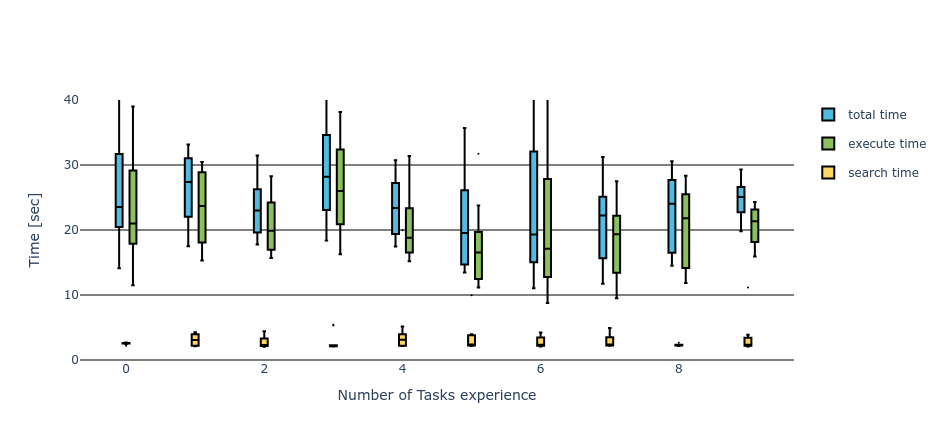
\includegraphics[width=\textwidth]{figures/results/random_drive_time_no_k-graph}
    \caption{Search-, execution- and total time to complete a drive task \textbf{without} \ac{k-graph} action suggestions and by randomly selecting edge parameterizations. The horizontal axis indicates the number of task experience in a run. The vertical axis displays a boxplot of the search-, execution- and total time over ten runs grouped by number of tasks in experience. }%
   \label{fig:random_drive_time_no_k-graph}
\end{figure}

When comparing the average median total time to complete a task in both \Cref{fig:random_drive_time_k-graph,fig:random_drive_time_no_k-graph} a difference becomes clear, which can be better visualized if only the medians of both task execution with and without the \ac{k-graph} action suggestions are plotted in the following figure.\bs

\begin{figure}[H]
    \centering
    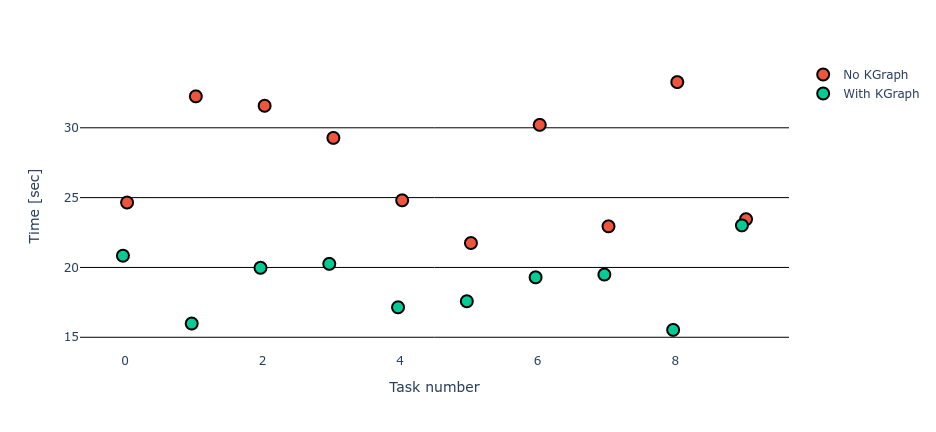
\includegraphics[width=\textwidth]{figures/results/random_drive_time_vs}
    \caption{Comparing means of total time to complete a task out of ten runs for a driving task.}\label{fig:random_drive_time_vs}
\end{figure}

In \Cref{fig:random_drive_time_k-graph} no clear trend could be indicated because the converging phase was over in the during the first task.When comparing the average medians for task execution with and without \ac{k-graph} action suggestions it becomes clear that the action suggestions result in a positive effect on the total time to complete a task. Without action suggestions the total time varies between 19 and 27 seconds, whilst task performance with action suggestions results in a total time that varies between 14 and 19 seconds. Now a table is presented that summarizes the edge parameterizations and displays success rate of tasks and hypotheses of the driving task.\bs

\begin{table}[H]
    \caption{The selection of the (\ac{MPC}, \textit{lti-drive-model}) parameterization versus selecting the (\ac{MPPI}, \textit{lti-drive-model}) parameterization for drive actions during the randomized driving tasks. The leftmost column indicates the metric to measure performance  with and without the \ac{k-graph} action suggestions. The rightmost column presents task performance over the number of tasks in experience.}%
    \label{table:rand_drive_mpc_vs_mppi}
    \centering
    \begin{tabular}%
      {%
        >{\raggedright\arraybackslash}p{0.10\textwidth}
        >{\raggedright\arraybackslash}p{0.22\textwidth}
      |p{0.4cm}p{0.4cm}p{0.4cm}p{0.4cm}p{0.4cm}p{0.4cm}p{0.4cm}p{0.4cm}p{0.4cm}p{0.4cm}}
      \multicolumn{2}{c|}{Number of Tasks in experience} &0&1&2&3&4&5&6&7&8&9\\\toprule
      \multirow{5}{0.1\textwidth}{With \ac{k-graph} suggestions} 
      &Number of \ac{MPC} parameterizations&20&30&31&31&30&30&31&30&30&33\\
      &Number of \ac{MPPI} parameterizations&10&0&0&0&0&0&0&0&0&0\\
      & task success rate [\%]& 100& 100& 100& 100& 100& 100& 100& 100& 100& 90\\
      & successfully hypothesis [-]& 30& 30& 30& 30& 30& 30& 30& 30& 30& 29\\
      & failed hypothesis [-]& 0& 0& 1& 1& 0& 0& 1& 0& 0& 4\\\midrule
      \multirow{5}{0.1\textwidth}{Without \ac{k-graph} suggestions} 
      &Number of \ac{MPC} parameterizations&12&14&13&10&15&16&13&17&16&9\\
      &Number of \ac{MPPI} parameterizations&18&17&18&20&17&15&17&13&15&22\\
      & task success rate [\%]& 100& 100& 100& 100& 100& 100& 100& 100& 100& 100\\
      & successfully hypothesis [-]& 30& 30& 30& 30& 30& 30& 30& 30& 30& 30\\
      & failed hypothesis [-]& 0& 1& 1& 0& 1& 1& 0& 0& 1& 1\\
    \end{tabular}
\end{table}

Whilst using the \ac{k-graph} suggestions the \ac{h-algorithm} almost completes all 300 (3 subtasks per task, 10 tasks per run, 10 runs are completed) driving subtasks. The 90\% success rate in the task using \ac{k-graph} suggestions and having 9 task in experience in \Cref{table:rand_drive_mpc_vs_mppi} can be assigned to pure chance, as it is a single occurrence. The \ac{h-algorithm} successfully completes 300 driving subtasks with random selection of edge parameterization. The number of \ac{MPC} and \ac{MPPI} parameterizations should be more or equal to 30 for any number of tasks in experience. In many cases it is more than 30, which indicates more than 30 drive edges were created to complete 30 drive subtasks. This effect is due to detected faults, that result in hypothesis failure. In such cases because two or more edge parameterization are initialized to complete a single subtask, that results in more than 30 driving edge parameterizations to complete 30 subtasks.\bs

For the driving task in the randomized environment the \ac{k-graph} converges to the (\textit{mpc-drive-controller}, \textit{lti-drive-model}) parameterization during the first task. Selecting this parameterization compared to selecting a random parameterization has a positive effect on the total time to complete a task. The search time for both using the \ac{k-graph} suggestions or random selection is similar. Now a similar experiment is conducted for a pushing task.\bs

\subsection{A Pushing Task}%
\label{subsec:rand_pushing}
The push task in the randomized environment consists of a single subtask. To complete this push task the robot must push the object toward its specified target pose. The tuning parameters that make up the random environment for the push task can be visualized in \Cref{table:configure_rand_push_env_values}.\bs

\begin{table}[H]
\caption{The selected tuning parameters for the randomized push environment.}%
\label{table:configure_rand_push_env_values}
\centering
\begin{tabular}%
{>{\raggedright\arraybackslash}p{0.30\textwidth}%
>{\raggedright\arraybackslash}p{0.60\textwidth}}
\text{grid size}  &\gls{x}=12 m, \quad \gls{y}=12 m \\
\text{object size}  &$\mathit{min\_length}=0.2 m, \quad \mathit{max\_length}=2 m$ \\
\text{object weight}  &$\mathit{max\_weight}=1000 g = 1 \mathit{kg}$\\
\text{number of objects}  &$\mathit{num\_unmovable\_obj}=3, \quad \mathit{num\_movable\_obj}=5$ \\
\text{number of tested runs}  &$\mathit{num\_runs}=10$\\
\text{number of tasks in a run}  &$\mathit{num\_tasks}=6$\\
\text{number of subtasks in a task}  &$\mathit{num\_subtasks}=1$
\end{tabular}
\end{table}

The available push edge parameterizations that can be selected are: (\textit{mppi-push-controller}, \textit{lti-push-model}) and (\textit{mppit-push-controller}, \textit{nonlinear-push-model}).\bs

\begin{figure}[H]
    \centering
    \begin{subfigure}{\textwidth}
    \centering
    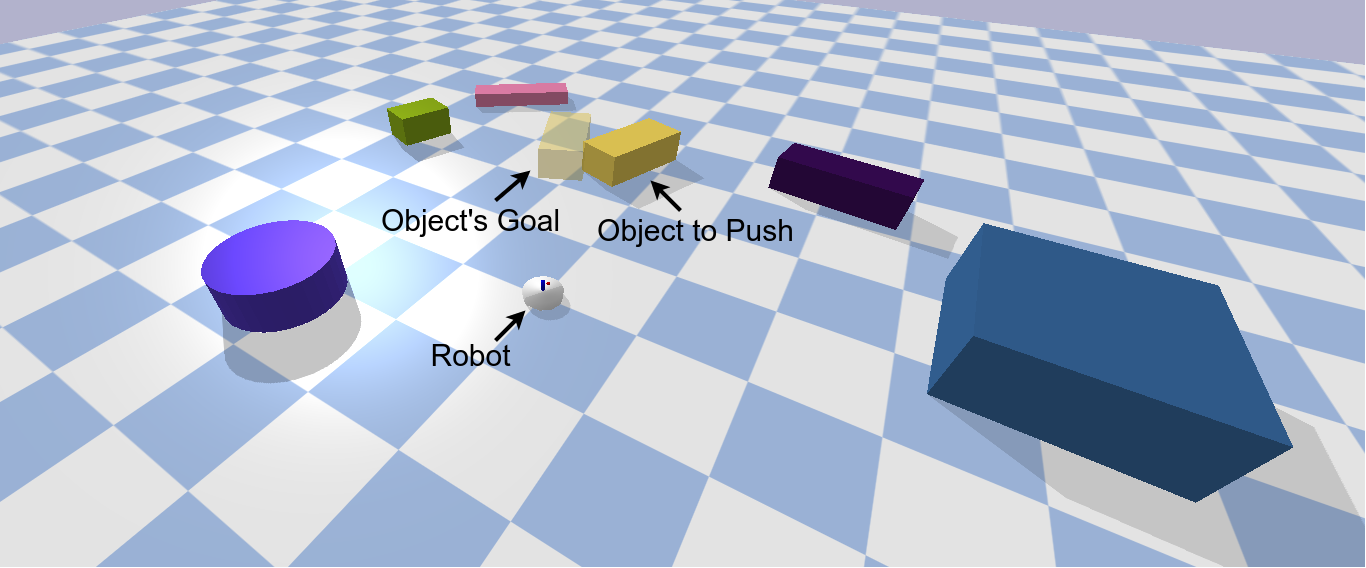
\includegraphics[width=0.9\textwidth]{figures/results/random_1.drawio}
    \caption{Robot tasked to push the yellow box toward the object's goal.}
    \end{subfigure}

    \vspace{0.2cm}
    \begin{subfigure}{\textwidth}
    \centering
    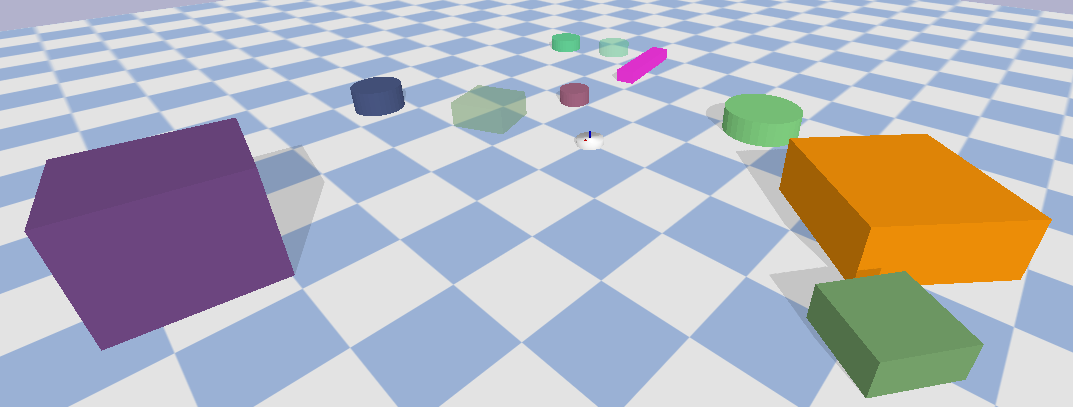
\includegraphics[width=0.9\textwidth]{figures/results/random_2}
    \caption{Robot tasked to push the brown box to the ghost pose.}
    \end{subfigure}
    \caption{Two random environments with the object's target displayed as a transparent ghost pose.}%
    \label{fig:random_environnment}
\end{figure}

Given the parameters range in table \Cref{table:configure_rand_push_env_values} randomized experiments are carried out for ten runs of pushing tasks. First the pushing tasks are completed using \ac{k-graph} suggestions. The search-, execute- and total time for task completion is presented in \Cref{fig:random_push_time_k-graph}. Then the same tasks are completed without help of the \ac{k-graph} suggestions in \Cref{fig:random_drive_time_no_k-graph}. 

\begin{figure}[H]
    \centering
    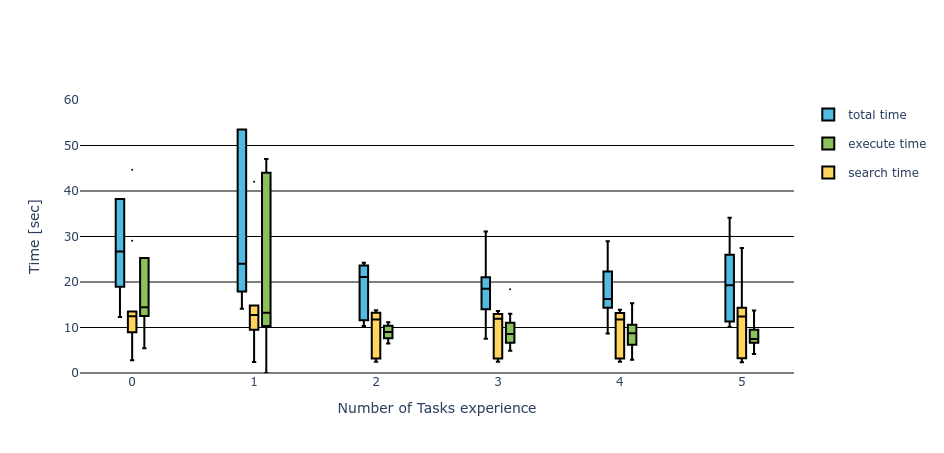
\includegraphics[width=\textwidth]{figures/results/random_push_time_k-graph}
    \caption{Search-, execution- and total time to complete a pushing task \textbf{with} \ac{k-graph} action suggestions. The horizontal axis indicates the number of task experience in a run. A run contains ten tasks, starting the run with an empty \ac{k-graph} that collects action feedback as the robot gains experience. The vertical axis displays a boxplot of the search-, execution- and total time over ten runs, where the sum of search- and execution time equals total time.}%
    \label{fig:random_push_time_k-graph}
\end{figure}

\Cref{fig:random_push_time_k-graph} above displays that the usage of the \ac{k-graph} lowers the total execution time with two tasks in experience. From \Cref{table:rand_push_model1_vs_model2} it can be concluded that the learning phase is over with two tasks in experience, since then only the parameterization with the \ac{LTI} model is selected when leveraging the \ac{k-graph}. A similar effect (total time to complete a task lowers after two tasks in experience) is then recorded in the following figure, that displays the results of the same tasks executed without action suggestions in \Cref{fig:random_push_time_k-graph}.\bs

\begin{figure}[H]
    \centering
    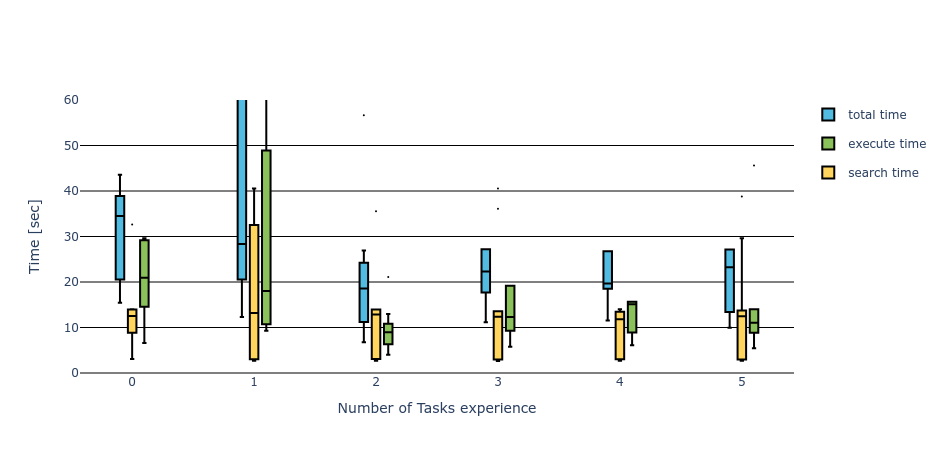
\includegraphics[width=\textwidth]{figures/results/random_push_time_no_k-graph}
    \caption{Search-, execution- and total time to complete a pushing task \textbf{without} \ac{k-graph} action suggestions. The horizontal axis indicates the number of task experience in a run. A run contains ten tasks, starting the run with an empty \ac{k-graph} that collects action feedback as the robot gains experience. The vertical axis displays a boxplot of the search-, execution- and total time over ten runs, where the sum of search- and execution time equals total time.}%
    \label{fig:random_push_time_no_k-graph}
\end{figure}

Both \Cref{fig:random_push_time_k-graph} and \Cref{fig:random_push_time_no_k-graph} look very similar due to solving the same tasks. Whilst gaining more experience the \ac{h-algorithm} that uses the \ac{k-graph} suggestions yields a better total task completion time. Which is easier to see if only the mean of the total tasks times are plotted in \Cref{fig:random_push_time_vs}. 

\begin{figure}[H]
    \centering
    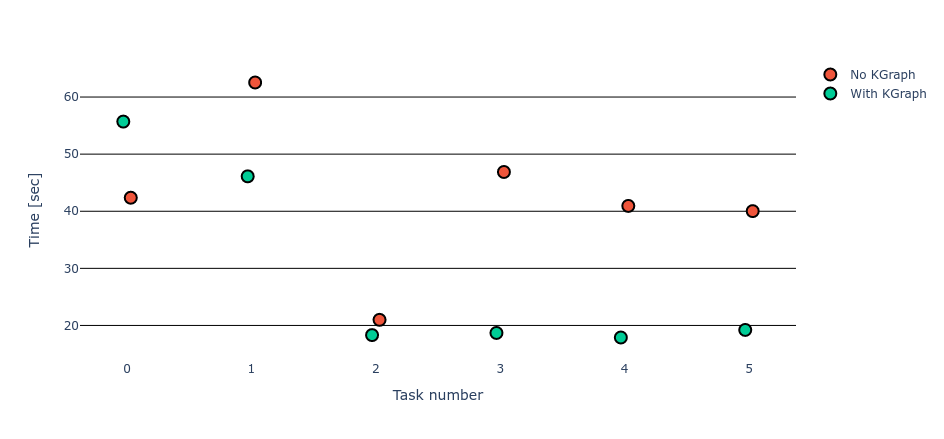
\includegraphics[width=\textwidth]{figures/results/random_push_time_vs}
    \caption{Comparing means of total time to complete a task out of ten runs for a pushing task.}\label{fig:random_push_time_vs}
\end{figure}

Both with and without action suggestion appear to lower total task execution time for pushing task, which begs the question: Is the trend in time to complete a task due to the \ac{k-graph} or due to chance?. Even if in both scenario's the total time lowers after two tasks in experience, there still is a small margin of difference if the action suggestions are used over random selection, which becomes clear when comparing average median task completion times in \Cref{fig:random_push_time_vs}.

\begin{table}[H]
    \caption{The selection of the (\ac{MPPI}, \textit{lti-push-model}) parameterization versus selecting the (\ac{MPPI}, \textit{nonlinear-push-model}) parameterization for push actions during the randomized pushing tasks. The leftmost column indicates the metric to measure performance  with and without the \ac{k-graph} action suggestions. The rightmost column presents task performance over the number of tasks in experience.}
    \label{table:rand_push_model1_vs_model2}
    \centering
    \begin{tabular}%
      {
        >{\raggedright\arraybackslash}p{0.10\textwidth}
        >{\raggedright\arraybackslash}p{0.35\textwidth}
      |p{0.4cm}p{0.4cm}p{0.4cm}p{0.4cm}p{0.4cm}p{0.4cm}}
      \multicolumn{2}{c|}{Number of Tasks in experience} &0&1&2&3&4&5\\\toprule
      \multirow{2}{0.1\textwidth}{With \ac{k-graph} suggestions} 
      &Number of \textit{lti-push-model} parameterizations&6&8&8&10&10&10\\
      &Number of \textit{nonlinear-push-model} parameterizations&7&9&2&0&0&0\\\hline
      % & task success rate [\%]& 90& 90& 100& 100& 100& 100\\
      % & successfully hypothesis [-]& 9& 9& 10& 10& 10& 10\\
      % & failed hypothesis [-]& 5& 8& 0& 0& 0& 0\\\midrule
      \multirow{2}{0.1\textwidth}{Without \ac{k-graph} suggestions} 
      &Number of \textit{lti-push-model} parameterizations&6&8&8&6&4&6\\
      &Number of \textit{nonlinear-push-model} parameterizations&8&9&3&6&6&8\\
      % & task success rate [\%]& 90& 80& 100& 100& 100& 90\\
      % & successfully hypothesis [-]& 9& 8& 10& 10& 10& 9\\
      % & failed hypothesis [-]& 5& 9& 1& 2& 0& 5\\
    \end{tabular}
\end{table}

The \ac{k-graph} favors the \ac{MPPI} controller with \textit{lti-push-model} as can be seen in \Cref{table:rand_push_model1_vs_model2}. The lti-push-model parameterization does not only have a lower execution time compared to the nonlinear-push-model parameterization, it also has a lower \ac{PE} as can be seen in \Cref{fig:random_push_pe_vs}. The difference in \ac{PE} between the \textit{lti-push-model} and the \textit{nonlinear-push-model} can be explained by involving a fixed geometrical property in the \textit{nonlinear-push-model}, which is the width of the object \textit{H} set to 2 meters. Just as with many solutions in general, a simple solution mostly works best.\bs

\begin{figure}[H]
    \centering
    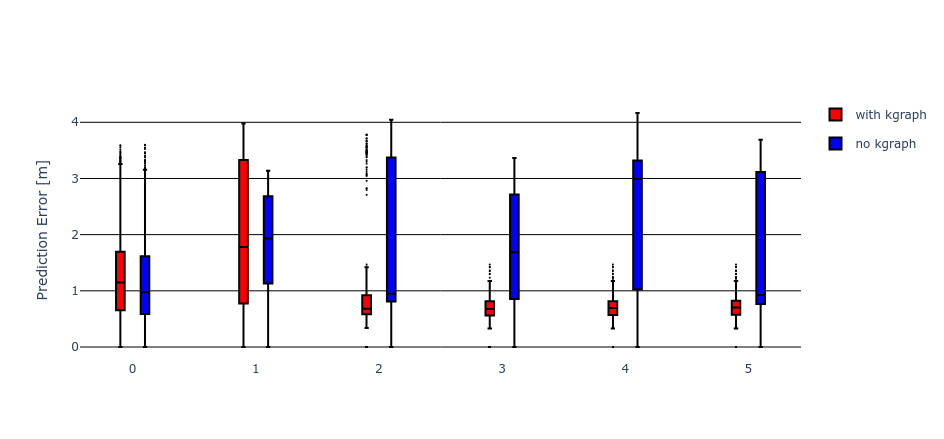
\includegraphics[width=\textwidth]{figures/results/random_push_pe_vs}
    \caption{Box plot of the \acl{PE} for solving reshuffled tasks. The horizontal axis indicates the number of task experience in a run. A run contains six tasks, starting the run with an empty \ac{k-graph} that collects action feedback as the robot gains experience. The vertical axis displays a boxplot of \acl{PE} over six runs. For the edge parameterizations once with the use of \ac{k-graph} action suggestions are leveraged indicated by \quotes{with \ac{k-graph}} and once with random selection indicated by \quotes{no \ac{k-graph}}.}%
    \label{fig:random_push_pe_vs}
\end{figure}

\Cref{fig:random_drive_time_vs,fig:random_push_time_vs,fig:random_push_pe_vs} all confirm that the use of the action suggestion provided by the \ac{k-graph} results in improved task total time and \ac{PE} compared to random selection of edge parameterizations. 

The strategy also named control and system model combination or edge parameterization to which the \ac{h-algorithm} converges is determined by two aspects. First, the set of available edge parameterizations, because the strategy can only converge toward the best available edge parameterization. Second, the success factor defined in \Cref{eq:success_factor}, because it determines which metrics play a role in selection of the best strategy. In this thesis the success factor favors an edge parameterization that bears a low \ac{PE} and thus, logically the \ac{k-graph} converges toward the edge parameterization with a lower \ac{PE}. Further investigation of different types of success factors are moved toward the future work section. Now the proposed framework is compared to the state-of-the-art in the upcoming section.\bs

\section{Comparison with State-of-the-Art}%
\label{sec:compare_with_related_papers}
A summary of state-of-the-art methods is presented again (as it was already presented in the introduction, \Cref{table:sota_and_3_topics}). The goal is now to highlight the test metrics the state-of-the-art methods used during their tests of their methods. Based on these, a fair test metric is used to compare with our approach.\bs

\noindent
\begin{table}[H]
\caption{Overview of recent state-of-the-art papers that include a subset of the 3 topics (learning system models, \ac{NAMO}, and nonprehensile pushing). The testing metric indicates the testing method used by the paper, where the underlined metric is used to compare against the proposed framework.}%
\label{table:sota_vs_results_proposed}
  \centering
  \rowcolors{2}{white}{myEvenLighterColor}
  \begin{tabular}
    {>{\raggedright\arraybackslash}P{1.5cm}%
      >{\raggedright\arraybackslash}P{1.0cm}%
      >{\centering\arraybackslash}P{1.4cm}%
      |>{\centering\arraybackslash}P{1.4cm}%
      >{\centering\arraybackslash}P{1.4cm}%
      |>{\centering\arraybackslash}P{1.4cm}%
      >{\centering\arraybackslash}P{1.4cm}%
      |>{\raggedright\arraybackslash}P{3.0cm}
    }
    &&& \multicolumn{2}{c|}{\ac{NAMO}} & \multicolumn{2}{c}{\shortstack[c]{Specify object\\target poses}}\\
  Author&
  Citation&
  Learns\newline object\newline dynamics&
  \vspace{-0.2cm}\rotatebox{50}{prehesile}&
  \vspace{-0.4cm}\rotatebox{50}{nonprehesile}&
  \vspace{-0.2cm}\rotatebox{50}{prehesile}&
  \vspace{-0.4cm}\rotatebox{50}{nonprehesile}&
  testing metric\\\toprule
  \citeauthor{ellis_navigation_2022} &          \cite{ellis_navigation_2022} &          \cmark& \xmark& \cmark& \xmark& \xmark& success rate\\
  \citeauthor{sabbaghnovin_model_2021} &        \cite{sabbaghnovin_model_2021} &        \cmark& \cmark& \xmark& \cmark& \xmark& success rate, execution time prediction error, final pose error\\
  \citeauthor{scholz_navigation_2016} &         \cite{scholz_navigation_2016} &         \cmark& \cmark& \xmark& \xmark& \xmark& runtime, planning time, number of replanning number of calls to update model\\
  \citeauthor{vega-brown_asymptotically_2020} & \cite{vega-brown_asymptotically_2020} & \xmark& \cmark& \xmark& \cmark& \xmark& computation time\\
  \citeauthor{wang_affordancebased_2020} &      \cite{wang_affordancebased_2020} & \cmark& \xmark& \cmark& \xmark& \xmark& \underline{computation and} \underline{execution time}\\
  Groote & Proposed Framework & \xmark/\cmark& \xmark& \cmark& \xmark& \cmark&
\end{tabular}
\end{table}

A comparison with a single state-of-the-art paper is made, that is accomplished by recreating the environment that the state-of-the-art has used during testing. With \citeauthor{wang_affordancebased_2020} the computation- (or search) and execution time is compared.\bs

% \paragraph{Comparing Success Rate with \citeauthor{ellis_navigation_2022}}
% \todo{This can use some extra review here, it is unclear}
% \citeauthor{ellis_navigation_2022} claims to push with a success rate \todo{Corrado: perhaps eleborate on that 100 percent, how does ellis define that?} of a 100\%~\cite{ellis_navigation_2022}. The test environment that \citeauthor{ellis_navigation_2022} has used is very similar to the random pushing task discussed in \Cref{sec:randomisation}. For both the random driving task and the random pushing task the success rate is 100\%. Meaning that every driving or pushing subtask was successfully completed. It is even so that for the result of the random push task (displayed in \Cref{fig:rand_push_full_pred,fig:random_push_all_times,fig:random_push_with_without_k-graph}) the number of hypotheses is equal to the number of subtasks \todo{Corrado: How do I see this? unclear to tthe reader}. Meaning that every subtask is completed by the first hypothesis generated. Both similar experiments from \citeauthor{ellis_navigation_2022} and this thesis have a 100\% success rate for similar
% , allowing us to conclude that the results are comparable.



% \paragraph{Comparing something TODO with \citeauthor{sabbaghnovin_model_2021}}
% \citeauthor{sabbaghnovin_model_2021} grasp-pushes and grasp-pulls a walker object to two new target configurations~\cite{sabbaghnovin_model_2021}. The task is mimicked by pushing a box object of equal dimensions to the same target configurations. Compared to \citeauthor{sabbaghnovin_model_2021} average of 125 and 160 seconds to complete task 1 and task 2 the proposed framework takes an average of only 27 and 33 seconds respectively (10 seconds computation time) to complete similar tasks. The decrease in total time allows to conclude that the proposed frameworks improve upon the method proposed by~\citeauthor{sabbaghnovin_model_2021}.\bs \todo{Corrado: So your pushing controllers are performin better than prehensile manipulation? amazing, but doub}



% \paragraph{Comparing something TODO with \citeauthor{vega-brown_asymptotically_2020}}
% \citeauthor{vega-brown_asymptotically_2020} has a task that pushes two boxes into a goal region. It takes around 300 seconds to return a hypothesis~\cite{vega-brown_asymptotically_2020}. \todo{Corrado: What do you mean? for the next sentce}Both pushing tasks can be compared with two separate pushing tasks from the random push environment. By doubling the time to push a single object to its target configuration, $2 \cdot 30 = 60$ seconds both tasks could be compared. However, the point of \citeauthor{vega-brown_asymptotically_2020} paper is that a global minimal task is sought. The proposed framework randomly selects a subtask and tries to complete it to then move to the next randomly selected subtask. A global minimum is thus not sought and both papers can therefore not be compared properly.\todo{Corrado: Then why including it in the comparison?}\bs



% \paragraph{Comparing Computation and Execution Time }
% Three state-of-the-art papers that use computation and execution time as the testing metrics are compared to the proposed framework. To accomplish a fair comparison the environments that have been used in the \todo{Corrado: Where do I see this?} citations are rebuilt in the pybullet software. The results are then directly compared to conclude that the proposed framework is as good as or even better in terms of computation time and execution time for similar tasks.\bs


\paragraph{Comparing Computation and Execution time with \citeauthor{wang_affordancebased_2020}}
\citeauthor{wang_affordancebased_2020} combines the \ac{NAMO} problem with learning object dynamics. \citeauthor{wang_affordancebased_2020} proposed framework takes an affordance approach than can be best described as: Affordance offers robots to perceive the environment in a way similar to humans do, by capturing the properties of objects without identifying them. The affordance approach is combined with a contact-implicit motion planning algorithm, a manipulation planning algorithm for push manipulation~\cite{wang_affordancebased_2020}. A test is performed in a real-world environment, where the robot drives toward a target pose, whilst the path is blocked by a chair. The real-world robot environment is implicitly represented as simulation environment. The environment is mimicked with three walls and a red box on the spot where is chair stands. The implicit representation of the real-world environment and the mimicked robot environments can be seen in \Cref{fig:wang}.\bs

\begin{figure}[H]
    \centering
    \begin{subfigure}{.49\textwidth}
    \centering
    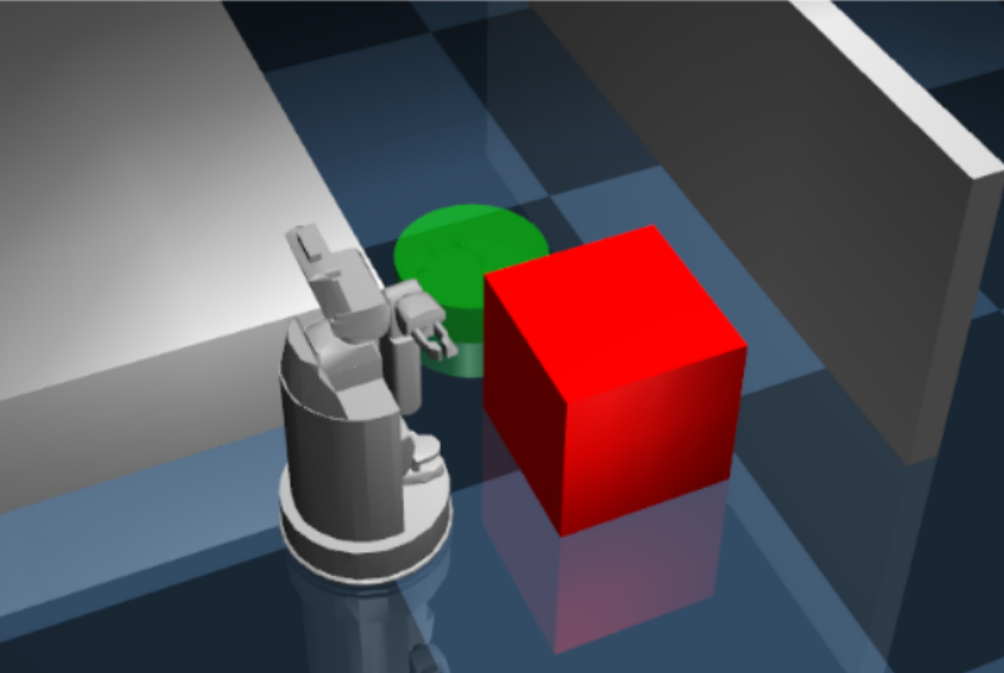
\includegraphics[width=0.9\textwidth]{figures/results/wang_env}
    \caption{\citeauthor{wang_affordancebased_2020} simulation environment.}%
    \label{subfig:wang_env}
    \end{subfigure}
    \hfill
    \begin{subfigure}{.49\textwidth}
    \centering
    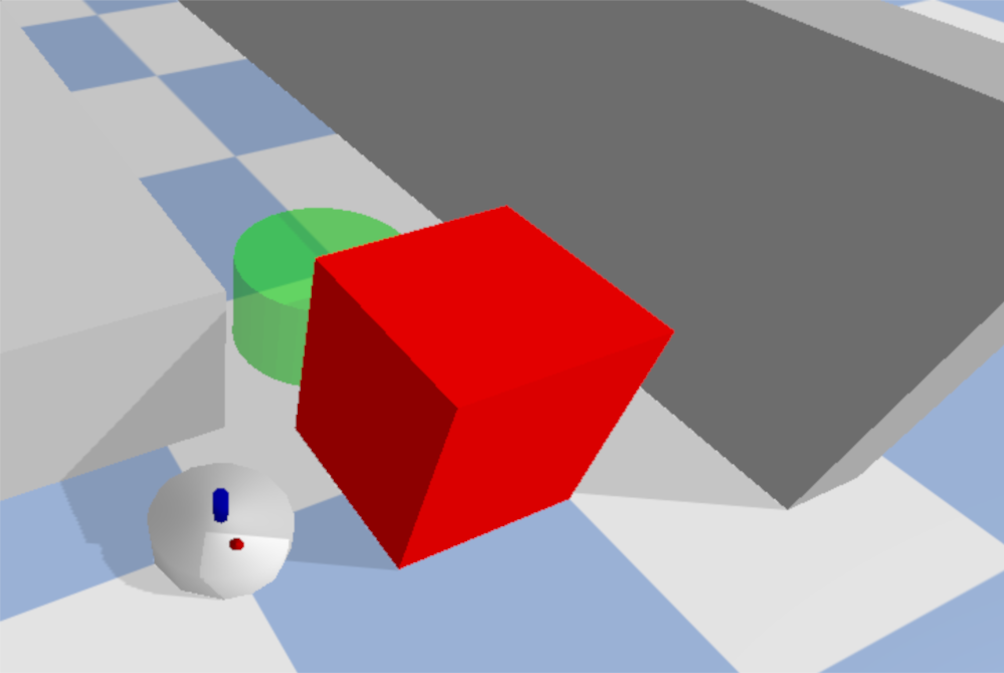
\includegraphics[width=0.9\textwidth]{figures/results/wang_mimick}
    \caption{Recreated robot environment.}%
    \label{subfig:wang_mimick}
    \end{subfigure}
    \caption{Two similar environments and tasks, the robots are tasked to drive toward a target pose indicated with the green ghost poses. In both environment a direct path is blocked by the red box.}%
    \label{fig:wang}
\end{figure}

\citeauthor{wang_affordancebased_2020} solves the task three times, the average search-, execute- and total time over these three executions is displayed in \Cref{table:wang_vs_mimick}. Note that, during testing \citeauthor{wang_affordancebased_2020} splits the search time in two categories; time to estimate accordance of an object and time to optimize the trajectory. For the purpose of comparison, we replicate the use case of \citeauthor{wang_affordancebased_2020} displayed in \Cref{subfig:wang_mimick}. The task is then solved ten times, every time starting without environmental knowledge and thus an empty \ac{k-graph}. The average search, execute- and total time over these then executions is also displayed in \Cref{table:wang_vs_mimick}.\bs

\begin{table}[H]
    \caption{Average execute-, search and total times for a task that involves learning object dynamics and the \ac{NAMO} problem. The results are average over three solved tasks for \citeauthor{wang_affordancebased_2020}, and ten solved tasks for the proposed framework. A visualization of the task if presented in \Cref{fig:wang}.}%
    \label{table:wang_vs_mimick}
    \centering
    \begin{tabular}%
    {>{\raggedright\arraybackslash}p{0.2\textwidth}|%
    >{\centering\arraybackslash}p{2cm}%
    >{\centering\arraybackslash}p{2cm}}%
    Author &\citeauthor{wang_affordancebased_2020} & Groote \\\toprule
    search time [sec]  & 109 & 26 \\
    execution time [sec]  & 67 & 4 \\
    total time [sec] & 176 & 30
    \end{tabular}
\end{table}

The proposed framework outperforms the contact-implicit motion planning framework proposed by \citeauthor{wang_affordancebased_2020}. Mainly the search time improves by a margin. The execution time improves, but because \citeauthor{wang_affordancebased_2020} tests in an real-world environment where motion equations are more complex compared to the simulated environment, an improvement in the execution time is expected.\bs

The test in randomized environments shows that edge parameterization selection based on experience in the environment improves task execution compared to random selection. Converging to a specific control method is influenced by the available control methods, and how the action feedback is calculated that forms the success factor. Comparison to a single state-of-the-art paper confirms that the \ac{h-algorithm} with the backward search is an effective tool to search and execute action sequences. Before claiming hard conclusions more tests should be performed for both converging toward an optimal controller and for the proposed method to complete tasks in unforeseen robot environments.\bs

% \paragraph{Comparing Prediction Error}
% \citeauthor{sabbaghnovin_model_2021} displays the final position errors for a selection of objects which range from 0.05 to 0.6 meters. A success threshold is set to 0.1 meters, which determines that the object is at its target location~\cite{sabbaghnovin_model_2021}. The success threshold in this thesis is set to a staggering 0.9 meters,\todo{Corrado: But then how can you compare success rate if you have different metrics for success?} thus it is concluded an object has reached its target position, whilst it is still 0.9 meters from its target configurations. This thesis does not try to reach optimal control, it tries to select the best controller in the available set of controllers. If the same controller from \citeauthor{sabbaghnovin_model_2021} would be available, then similar final position errors would be obtained. It can be concluded that the prediction error \todo{Corrado: Not position errro?}of the proposed framework is worse compared to this state-of-the-art. The reason is that the proposed framework focuses on improving the control selection and action sequences over time, and not on lowering final prediction errors.\bs

% \paragraph{Comparing Number of Replanning times}
% \todo[inline]{\cite{scholz_navigation_2016}}
% \todo{recreate this envionrment, run 10 tests and compare the search and execution time, as well at the number of call toward the planner}
% \todo{additinoally execute this environment a twice in a row, show that the execution number of call to the planner drops, theand the execution time drops}
